\label{sec:conclusions}

The objective of this research project is to provide a definitive
assessment of the technological feasibility of the entire synthetic
columnar vortex concept as a means of generating usable energy. In the 
previous sections outlined the present state of the
simulation capability. In doing so, we have discussed the physics that
influence dust devils formation, our particular mathematical
models for the ambient conditions, as well as the SoV vanes, cone and
turbine. We summarized the numerical discretizations used, the software
stack and the calibration, verification and validation of these
components. The purpose of these sections was to communicate
two major points. The first is that an accurate, verified and
validated simulation capability has been developed that can quickly
investigate a wide variety of system and scenario settings at a modest
computational cost. The second point is that we have developed
heuristics that permit optimization of any baseline SoV configuration to
a local maximum of energy production, as measured by kinetic energy flux
through the top of the SoV vanes.  

These two points justify the proposed course of work, which is to
explore a large space of possible system configurations
and geometries to discover the globally optimal structure
of the SoV apparatus. Coupled with the scaling analysis presented in
Section \ref{sec:physics}, we will then be able to predict the
conditions (if any) under which the SoV apparatus will be
technologically feasible. This will lead to investigating the physics of the
apparatus, to assess how closely the synthetic dust devils mimic the
natural variety. The proposed research is designed to
assess feasibility, and it is not expected that actual experimental
validation will accompany the computational results. Furthermore, it
must also be emphasized that feasibility is focused on
technical viability, namely energy produced by the apparatus,
and will not include an economic assessment. In other words, it is
possible that the SoV will produce energy, but the design required to do
is prohibitively expensive, and therefore not economically competitive
with existing technologies. The following is a proposed program of simulations 
designed to explore a wide configuration space. This focuses on
optimization for the cone, turbine and vanes. 

%
% vane optimization
%
%% \large
%% \begin{center}
%% \begin{table}[h]
%%  \centering
%%   \begin{tabular}{| l | c | l |}
%%     \hline
%%     Parameter & Description & Range \\
%%     \hline
%%     $\theta^{\text{t}}_{\text{min}}$ & Starting, minimum angle of the
%%        top tier & ( 0 - $\theta^{\text{t}}_{\text{max}}$ ) \\
%%     $\theta^{\text{t}}_{\text{max}}$ & Ending, maximum angle of the top
%%        tier & ( 0 - 90 ) \\
%%     $\theta^{\text{b}}_{\text{min}}$ & Starting, minimum angle of the
%%        bottom tier & ( 0 - $\theta^{\text{b}}_{\text{max}}$ ) \\
%%     $\theta^{\text{b}}_{\text{max}}$ & Ending, maximum angle of the
%%        bottom tier & ( 0 - 90 ) \\
%%    $\gamma^t$ & Rate of curving, vane top tier & ( 0 - 3 ) \\
%%    $\gamma^b$ & Rate of curving, vane bottom tier & ( 0 - 3 ) \\
%%    $1 - (r_{\text{min}} / r_{\text{max}})^{\text{t}}$ & Length of the top
%%        tier vane & ( 0 - 1 ) \\
%%    $1 - (r_{\text{min}} / r_{\text{max}})^{\text{b}}$ & Length of the
%%        bottom 
%%        tier vane & ( 0 - 1 ) \\
%%    $H^b/H^t$ & Ratio of heights between bottom and top tiers & ( 0 -
%% 	   0.5 ) \\ 
%%    $D/H$ & Ratio of apparatus diameter and total vane height & ( 0.5 -
%% 	   5.0 ) \\ 
%%     \hline
%%   \end{tabular}
%%   \caption{Vane Optimization Parameters.}
%%   \label{tab:vane}
%% \end{table}
%% \end{center}
%% \normalsize\todo{keep table?}

The three cone parameters we propose to optimize are shown in Table
\ref{tab:cone}. We expect to optimize the cone after the bottom and top
tiers are adjusted. For the cone, we expect the height, maximum diameter
and inner exit diameter to all impact the flow. While it is not known
what form the ideal cone geometry will take, our expectation is that the
cone plays at least two important roles. The first is acting as a
converging nozzle for the flow, increasing the vertical and azimuthal
velocity as it exits out the top of the device. In the wind, the cone
also acts as a shield, preventing the high velocity freestream flow from
disrupting the vortex before it has run through the turbine. 

%
% cone optimization
%
\begin{center}
\begin{table}[h]
 \centering
  \begin{tabular}{| l | c | l |}
    \hline
    Parameter & Description & Range \\
    \hline
    $H_C/D_C$ & Ratio of the height of the cone versus the cone diameter & ( 0 - 2.0 ) \\
    $D_{\text{C}}/D$ & Ratio of the cone diameter versus the system
       diameter & ( 0.5 - 1.5 ) \\
    $D_{\text{out}}/D_C$ & Ratio of the cone exit diameter versus the
       cone diameter & ( 0.25 - 1.0 ) \\ 
    \hline
  \end{tabular}
  \caption{Cone Optimization Parameters.}
  \label{tab:cone}
\end{table}
\end{center}

The turbine parameters to be optimized are shown in Table
\ref{tab:turbine}. In addition to these configuration parameters, the
location of the turbine will likely need to be optimized to be centered
on the vortex, which may not be centered inside the vanes due to
asymmetric effects of wind, vane geometry, etc. 

%
% turbine optimization
%
\begin{center}
\begin{table}[h]
 \centering
  \begin{tabular}{| l | c | l |}
    \hline
    Parameter & Description & Range \\
    \hline
    $N_B$ & Number of blades & ( 1 - 12 ) \\
    $I$ & Moment of inertia & ( 1 - 12 ) \\
    $r_B/r_{\text{min}}^t$ & Radius of blade versus the inner radius of
       the top tier vanes & ( 0 - 1 ) \\
   $H_B/H$ & Height of the turbine blades versus system height & ( 0 - 1.2 ) \\
    \hline
  \end{tabular}
  \caption{Proposed Turbine Optimization Parameters.}
  \label{tab:turbine}
\end{table}
\end{center}

The possible configuration space for the vanes is much larger. 
Presently, the workflow consists of weekly calls with the experimental
team to discuss possible system designs, which typically consist of vane
sketches or drawings. One such proposed design is shown in Figure
\ref{fig:sketch}.  These vanes are highly asymmetric with variation in
the length and curvature as a function of spatial location. Furthermore,
in this design the down wind side of the apparatus is enclosed by a
solid cylindrical wall.  While the vane representation outlined in
Section \ref{subsec:vane} is expected to be sufficiently general to support a
wide variety of vane configurations, it is not at this time clear what
form of parameterization for vane angle is sufficiently general to
support this exploration, and so a table like that for the cone and
turbine is not yet available. At present the expectation is to proceed
with this conceptual phase to generate a wide  range of possible
configurations. The designs that have initially promising results will
then be optimized similar to the examples outlined in Section
\ref{sec:results}, where new parameter values are 
introduced, a run is performed, and then the output is postprocessed and
evaluated before the process begins again. In this way it is not
infeasible to expect that several hundred optimization runs can be
performed. 
%The next subsection also briefly outlines a proposal to
%investigate algorithmic optimization on these designs.  

\begin{figure}[htb]
 \centering
 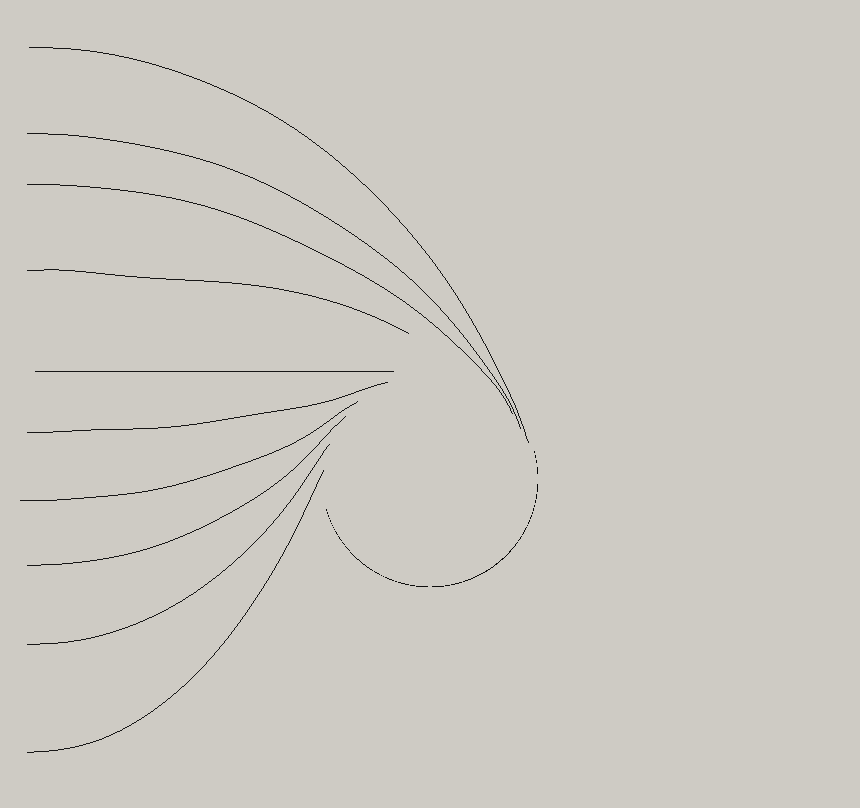
\includegraphics[width=.75\linewidth]{figs/top}
 \caption{This is an example image of a proposed vane design. The lines
 indicate the vane curvature and solid surfaces. Sketches and diagrams
 such as this  are typically generated by various members of the
 team. The vane surface is then instantiated as a region of forcing as
 detailed in Section \ref{subsec:vane} and then simulated. If the
 initial results are promising, then further exploration of that
 configuration may be pursued.} 
 \label{fig:sketch}
\end{figure}



% Table \ref{tab:vane} lists the proposed optimization parameters for the
% vanes. We propose nine parameters to optimize for the
% vanes. $\theta^{\text{t}}_{\text{min}}$ and
% $\theta^{\text{b}}_{\text{min}}$ are the top and bottom tier minimum
% angles. This is essentially the starting (and minimum) angle for the curved
% vanes. Preliminary investigations have given no indication that the
% bottom tier is receptive to anything but a fully radial angle
% (e.g. $0^{\circ}$). For the top tier, however, a non-zero
% $\theta_{\text{min}}$ has been found to increase the kinetic energy
% flux. For both of the maximum angles we have reasonable starting
% points. Previously, we have found that a larger angle at the bottom tier
% is ideal, as it serves to ``spin-up'' a small core region.

% We have less strongly informed prior expectations of reasonable values
% for the rate of curvature, $\gamma$, the ratio of heights between the
% top and bottom tiers ($H^b/H^t$) as well as the lengths of the
% vanes. The generated flux is certainly sensitive to $\gamma$, but
% optimal value is certainly not known. Likewise, while we have operated
% with shorter vanes lengths on the top than the bottom, as well as a
% shorter height, we are not certain that these configurations are
% remotely optimal. Finally, for $D/H$, the ratio between the apparatus
% diameter and total vane height, we have only operated near a ratio of
% 1.0. However, as noted in \cite{ROG:ROG1635}, ``Most dust devils are at 
% least 5 times higher than they are wide''. While increasing the height
% of the apparatus would greatly increase the cost and inaccessibility of
% the device for maintainance, this indicates that it is necessary to
% examine the dependence of energy produce by the vortex at greater system
% heights. We expect to increase beyond this aspect ratio of $\approx 1$
% towards the naturally occuring ratio of 5. If this is found to greatly
% enhance energy output, we will then consider even larger
% ratios.\todo{add image}
%
% need to expand this to discuss huge space of vanes
% add image too?
%



%\subsection{Risks and Challenges to the Optimization Efforts}

%% A challenge inherent to this optimization effort is that while the
%% principle quantity of interest is the kinetic energy flux, we also seek
%% to use these runs to shed light on the mechanisms by which the apparatus
%% configuration dictates the flow. In other words, we are trying learn
%% more than \textbf{which} configurations optimize the flow, but also 
%% \textbf{why} they do so. 

% This presents an programmatic challenge, as
% optimization will involve additional analysis and postprocessing at each
% iteration.  

%
% how many runs are we capable of performing, realistically
% largely obsolete!

% An additional challenge is the computational expense of each run. 
% Each parameter exploration requires approximately 12 wall-clock hours to run
% the simulation for a sufficient time to pass any initial transient in
% the solution and then permit adequate statistical averaging at steady
% state. Runs generally require approximately 264 processors on Lonestar
% (for example) and therefore the cost of a forward run is $\approx 3,200$
% core hours. Our overall compute budget will likely be between one hundred
% thousand to one million core hours. In other words, our present
% computational budge will support running between roughly 30 to 300
% instances for our parameter sweeps. While this is not insubstantial, this
% is not a sufficient number of evaluations to support formal
% optimization algorithms. While we admittedly do not, \textit{a priori},
% know the number of iterations necessary to solve the system, as it is
% non-linear, our expectation is that thousands of forward solves would be
% necessary. Using higher order methods could reduce the number of
% iterations, but gradient and derivative information is difficult to
% access, as solving the adjoint problem is expensive for unsteady systems. 
% Thus, while any individual run is relative inexpensive, we do not expect
% to be able to mount an exhaustive campaign to formally optimize the
% configuration given the dimension of the parameter space and the
% structure of the problem. 

%
% introduce concept of subdomains
%

% Furthermore, the time requires to perform this simulation campaign could
% be greatly reduced if several problems were to be undertaken in
% parallel. This ``divide and conquer'' approach requires subdividing the
% optimization effort into several ``subdomains''. 
% The problem is nonlinear, and so some of the parameters are coupled and
% cannot be easily optimized independent of each another, as adjustments
% to one impact the desired value of the other. 
% We propose to subdivide the vanes into upper and lower tiers, optimize
% them individually, and then perform rudimentary sensitivity checks to
% ensure that the coupled product does in fact represent a near optimal
% flux output. We further expect that the remaining parameters in the
% vanes, namely $H^b/H^t$, $D/H$ are amenable to optimization independent
% of the particular parametric configuration of the vane tiers. 

% The subdomains for the vanes are are summarized in Table
% \ref{tab:opt}. This neatly divides the vane optimization effort into
% three independent problems with 4 or fewer parameters each.

% \begin{center}
% \begin{table}[h]
%  \centering
%   \begin{tabular}{|l | l | l |}
%    \multicolumn{3}{c}{Subdomains} \\
%     \hline
%    Top Tier & Bottom Tier & Misc. \\
%    \hline
%    $\theta^{\text{t}}_{\text{min}}$ & $\theta^{\text{b}}_{\text{min}}$ &
%        $H^b/H^t$ \\
%    $\theta^{\text{t}}_{\text{max}}$ & $\theta^{\text{b}}_{\text{max}}$&
% 	   $D/H$ \\ 
%    $\gamma^t$ & $\gamma^b$ & \\
%    $1 - (r_{\text{min}} / r_{\text{max}})^{\text{t}}$ & $1 -
%        (r_{\text{min}} / r_{\text{max}})^{\text{b}}$ & \\
%    \hline
%   \end{tabular}
%   \caption{Vane optimization parameters, divided into parallelizable
%  subdomains.} 
%   \label{tab:opt}
% \end{table}
% \end{center}

\subsection{Proposed Timeline}

%
% timeline
%
A timeline for the proposed work is presented in Table
\ref{tab:prop}. The date of each bullet is the planned completion of the
deliverable. Bullets items in black are required, while those in blue
are optional, and do not need to be completed to ensure the
success of this project. 

% 
% can we optimize? DAKOTA
% 
% We propose to investigate algorithmic optimization as a tool to discover
% locally optimal system configurations. 
% This will take the form of using either the DAKOTA\cite{adams2013dakota}
% or TAO\cite{tao-user-ref} libraries. These libraries have suites of
% algorithms for non-linear optimization problems without gradient
% information (derivative-free optimization, such as Nelder-Mead or downhill simplex methods). 
% Evaluating the results of the most
% appropriate ``out of the box'' available optimization algorithm on a
% small test problem will provide an opportunity to ensure that our
% expectations on the number of iterations necessary for formal
% optimization of our problem are reasonably correct. 
% We propose these two libraries because DAKOTA is well-known as a library
% with extensive ``black-box'' optimization support, and TAO is already
% made available through pre-existing libMesh dependencies. Should the
% test problem discover that algorithmic optimization is a viable option,
% we will consider using this approach for optimization of the
% configuration. 

%
% short summary of tasks
%

The first bullet in Table \ref{tab:prop} provide
estimated ending dates for the exploration of the configuration space. 
We have rapidly iterated 
through these optimization efforts over the course of several
months, and are nearly converged on a final design. 
The second bullet relates to the the final verification of the turbine, to ensure
this functions properly. 
At this time we will proceed with ``coupling tests'' to 
ensure that the parameters are indeed still appropriate. For example,
after having optimized the turbine parameters, it may be necessary to
perturb the lower tier vane parameters to ensure that the selected set
is nearly optimal even with the addition of a turbine. 

%
% probably ok below:
%
The third bullet is the expected deadline to provide the results of our
computational simulation efforts to the experimental group in late
Spring/early Summer of 2016 so that they can use this information in the
design of the system to be used for the Arizona field tests in Summer,
2016. The date of the actual field test has not yet been set and may change. 

As mentioned in the fourth item, it is possible that this
project will permit some glimpses  
at the fundamental processes underlying the naturally dust devil
phenomena. To accomplish this, the synthetic dust devils must be
compared to data from the naturally occuring variety,  with some
appropriate scaling. While it is not a significant component of the
proposal, this and several simple investigations into related phenomena
such as tornados and hurricanes will also  be investigated. A literature
review of the physics of general cyclonic structures and any observed
intensification mechanisms may provide hints of the geometries 
by which the flow is intensified, and why. 

Given our previous experiences, we do not anticipate a rich validation data set 
to be available after the field test. Nevertheless, we will postprocess any and all
available data from this event in order to assess the reliability of the computational
modeling efforts. 

Finally, we anticipate a detailed accounting of the entire project as
the final deliverable. We expect that all of the investigations detailed 
above will result in several publications, as well. 

%
% itemize tasks
%
% In summary, in addition to the preliminary results, several tasks will be
% accomplished  to fulfill the goals of this project:

% \begin{itemize}
%  \item validate turbine
%  \item numerous optimization runs
%  \item best guess of ideal run (possible field run)
%  \item feasibility study?
% \end{itemize}

\begin{center}
\begin{table}
\caption{Timeline of proposed work. Bullets are dates of planned
 completion of deliverables. Black items are requisite, blue optional.}
\centering
\begin{minipage}[t]{.7\linewidth}
\color{black}
\rule{\linewidth}{1pt}
\ytl{April 2016}{Conclude parameter sweeps and optimization of apparatus}
\ytl{April 2016}{Turbine actuator-disk verification, validation and prediction}
\ytl{May 2016}{Proposed configuration and predictions for experimental
 team}
\ytb{July 2016}{Comparisons between synthetic and natural dust devil physics}
\ytl{Aug 2016}{Validation against 2016 field data}
%\ytl{Aug 2016}{SoV feasibility assessment}
\ytl{Fall 2016}{Doctoral dissertation writing}
\bigskip
\rule{\linewidth}{1pt}%
\end{minipage}%
\end{table}
\label{tab:prop}
\end{center}

% \subsection{Additional Investigations}

% % 
% % control for inter unit spacing
% % 
% In addition to the system configuration, it would be interest to consider the
% effect of local conditions on SoV performance. Characterizing the impact
% of variations in ambient conditions on the SoV will guide the
% commercialization strategy of the product, by determining optimal
% install locations across the country. It is therefore desirable to have
% models that are capable of accounting for variation in field conditions,
% such as solar input, cross-winds and topography. Furthermore, it is
% expected that large ``farms'' of SoVs (akin to the wind and solar farms
% for wind turbines and photovoltaics, respectively) may be used by
% commercial or utility-scale energy generation. For this to be
% effective,  the inter-unit spacing must also be optimized, as a single
% SoV collects from a large area. These computations will guide
% commercialization planning, where decision-makers will need to assess
% optimum unit size, spacing, and geographic location for utility-scale
% deployment.   
